\documentclass[conference]{IEEEtran}
\IEEEoverridecommandlockouts
% The preceding line is only needed to identify funding in the first footnote. If that is unneeded, please comment it out.
\usepackage{cite}
\usepackage{hyperref}
\usepackage{amsmath,amssymb,amsfonts}
\usepackage{algorithmic}
\usepackage{graphicx}
\usepackage{textcomp}
\usepackage{xcolor}
\usepackage{pgfplots, pgfplotstable}
\pgfplotsset{compat=1.18}

% ======= START: Plot for Reward-Epsilon progress =========
\newcommand{\rlplot}[5]{
% Parameters: 
% #1 = CSV file path
% #2 = Figure caption
% #3 = Figure label
% #4 = Y-axis min for rewards
% #5 = Y-axis max for rewards
\begin{figure}[htbp]
\centering

% Read the data (skip first 6 lines is hard-coded)
\pgfplotstableread[
    col sep=comma,
    skip first n=6
]{#1}\tempdatatable

\begin{tikzpicture}
\pgfplotsset{
    scale only axis,
    width=0.75\columnwidth,
    height=5cm
}

\begin{axis}[
    xlabel={},
    ylabel={Total Reward},
    ylabel style={color=blue!30},
    ymin=#4, ymax=#5,
    axis y line*=left,
    grid=major,
    tick label style={font=\tiny},
    label style={font=\footnotesize}
]
\addplot[color=blue!30, thick, smooth] 
    table[x=Episode, y=TotalReward] {\tempdatatable};
\end{axis}

\begin{axis}[
    xlabel={},
    ylabel={Epsilon $\varepsilon$},
    ylabel style={color=red},
    ymin=0, ymax=1,
    axis y line*=right,
    axis x line=none,
    tick label style={font=\tiny},
    label style={font=\footnotesize}
]
\addplot[color=red, thick, smooth] 
    table[x=Episode, y=Epsilon] {\tempdatatable};
\end{axis}
\end{tikzpicture}

% Custom x-label with legend
\noindent\footnotesize
Episode \qquad
\textcolor{blue!30}{\rule{6pt}{1pt}} Reward \quad
\textcolor{red}{\rule{6pt}{1pt}} Epsilon $\varepsilon$

\caption{#2}
\label{#3}
\end{figure}
}
% ======= END: Plot for Reward-Epsilon progress =========

\def\BibTeX{{\rm B\kern-.05em{\sc i\kern-.025em b}\kern-.08em
    T\kern-.1667em\lower.7ex\hbox{E}\kern-.125emX}}
\begin{document}

\title{Interactive Reinforcement Learning\\
{\footnotesize A Browser-Based Environment for Educational Q-Learning Visualization}
}

\author{\IEEEauthorblockN{Jakob Johannes Garde}
\IEEEauthorblockA{jgard22@student.sdu.dk}}

\maketitle

\begin{abstract}
Reinforcement learning education faces significant challenges as students struggle to understand abstract concepts like exploration-exploitation trade-offs through mathematical formulations alone. Traditional approaches require complex programming environments and non-real-time training, obscuring fundamental principles. This paper presents a browser-based Q-learning environment enabling real-time visualization of learning behavior with simplified parameter control.

The system implements a navigation task where an agent learns to reach a goal while avoiding obstacles, using tabular Q-learning with user-controllable learning rate, discount factor, exploration rate, and reward structure. The web interface provides immediate observation of learning dynamics without programming requirements, featuring real-time monitoring, dynamic obstacle toggling, and data export capabilities.

The system successfully bridges theoretical reinforcement learning concepts with intuitive understanding through accessible visualization and parameter manipulation, validating the educational value of simplified, real-time learning environments.

\href{https://jakobjgarde.github.io/reinforced/}{\color{blue}\textit{Link to online demo}}. - NOTICE: The demo has not been adapted to smaller screensizes (smartphones), so it is recommended to use a desktop or laptop computer for the best experience.
\end{abstract}

\section{Introduction}

Reinforcement learning represents one of the most conceptually challenging areas within machine learning education. While the mathematical foundations of Markov Decision Processes and temporal difference learning are well-established, students often struggle to develop intuitive understanding when confronted solely with equations and algorithmic descriptions. The abstract nature of concepts such as value functions, policy optimization, and the exploration-exploitation trade-off becomes particularly difficult to grasp without direct observation of the learning process in action.

Traditional reinforcement learning education compounds these challenges through reliance on complex programming environments and non-real-time training paradigms. Students typically encounter reinforcement learning through frameworks such as Gymnasium, where implementation requires substantial Python programming expertise and familiarity with machine learning libraries. Training processes often demand GPU acceleration and extended computation times, leaving students to interpret learning progress through post-hoc analysis of performance graphs and numerical metrics rather than observing the dynamic decision-making process as it unfolds.

Furthermore, production-level reinforcement learning implementations expose learners to overwhelming parameter spaces, with dozens of hyperparameters and architectural choices that obscure fundamental learning principles. This complexity creates significant cognitive overhead, preventing students from focusing on core concepts such as how learning rate affects the speed of learning, how discount factor influences long-term planning, and how exploration strategies impact discovery of optimal behaviors.

This work addresses these pedagogical limitations through the development of a browser-based, real-time reinforcement learning environment that prioritizes conceptual understanding over implementation complexity. By providing immediate visual feedback, interactive parameter control, and a simplified interface that exposes only essential learning components—learning rate, discount factor, exploration rate, and reward structure—the system enables students to observe and understand reinforcement learning behavior without the barriers typically associated with traditional educational approaches.
\section{Literature Review}

\subsection{Theoretical Foundations}

\subsubsection{Markov Decision Processes}
Reinforcement learning problems are formally modeled as Markov Decision Processes (MDPs), a mathematical framework first introduced by Bellman \cite{bellman1957} for sequential decision-making under uncertainty. An MDP is defined by the tuple $(S, A, P, R, \gamma)$, where $S$ represents the state space, $A$ the action space, $P$ the transition probability function, $R$ the reward function, and $\gamma$ the discount factor \cite{sutton2018reinforcement}.

The fundamental assumption underlying MDPs is the Markov property, which states that the future state depends only on the current state and action, not on the sequence of events that led to the current state.

The objective in an MDP is to find an optimal policy $\pi^*$ that maximizes the expected cumulative discounted reward:

\begin{equation}
\pi^* = \arg\max_\pi \mathbb{E}\left[\sum_{t=0}^{\infty} \gamma^t R_t | \pi\right]
\end{equation}

where $\gamma \in [0,1]$ is the discount factor that determines the relative importance of immediate versus future rewards.

\subsubsection{Value Functions and Bellman Equations}
The solution to MDPs relies on value functions that estimate the expected return from a given state or state-action pair. The state-value function $V^\pi(s)$ represents the expected return when starting from state $s$ and following policy $\pi$:

\begin{equation}
V^\pi(s) = \mathbb{E}_\pi\left[\sum_{k=0}^{\infty} \gamma^k R_{t+k+1} | S_t = s\right]
\end{equation}

Similarly, the action-value function $Q^\pi(s,a)$ represents the expected return when starting from state $s$, taking action $a$, and subsequently following policy $\pi$:

\begin{equation}
Q^\pi(s,a) = \mathbb{E}_\pi\left[\sum_{k=0}^{\infty} \gamma^k R_{t+k+1} | S_t = s, A_t = a\right]
\end{equation}

The Bellman equations provide recursive relationships for these value functions, forming the theoretical foundation for dynamic programming approaches to solving MDPs \cite{bellman1957}.

\subsection{Q-Learning Algorithm}
Q-learning, introduced by Watkins \cite{watkins1992q}, is a model-free reinforcement learning algorithm that learns the optimal action-value function without requiring knowledge of the environment's transition probabilities or reward function. The algorithm directly estimates $Q^*(s,a)$, the optimal action-value function, through temporal difference learning.

The Q-learning update rule combines immediate reward information with estimates of future value:

\begin{equation}
Q(s,a) \leftarrow Q(s,a) + \alpha \left[r + \gamma \max_{a'} Q(s',a') - Q(s,a)\right]
\end{equation}

where $\alpha$ is the learning rate controlling the magnitude of updates.

\subsection{Exploration in Reinforcement Learning}
The exploration-exploitation dilemma is central to reinforcement learning, requiring agents to balance between exploiting current knowledge and exploring potentially better alternatives \cite{thrun1992efficient}. The $\varepsilon$-greedy strategy, employed in this study, provides a simple yet effective approach by selecting random actions with probability $\varepsilon$ and the greedy action otherwise \cite{sutton2018reinforcement}.

\subsection{Educational Applications of Reinforcement Learning}

Gymnasium \cite{gymnasium2023}, maintained by the Farama Foundation, represents the current standard for reinforcement learning environments, providing a comprehensive collection of benchmark problems. However, these environments often require significant programming expertise and familiarity with Python ecosystems, potentially creating barriers for students new to both programming and reinforcement learning concepts.
\section{Method/Implementation}

\subsection{Technical Setup}

The experimental environment was developed using React, a JavaScript library for building user interfaces, in combination with React Three Fiber (R3F), a React renderer for Three.js that enables declarative 3D scene construction in web browsers. This technology stack was chosen to create an accessible, browser-based reinforcement learning environment that requires no specialized software installation, making it suitable for educational purposes and broad accessibility.

The application architecture separates the game environment from the learning algorithm, allowing for both manual control through keyboard inputs and autonomous operation via the reinforcement learning agent. State management was implemented using Zustand, a lightweight state management solution, to handle real-time parameter adjustments and data collection throughout the training process.

\subsection{Environment Design}

\subsubsection{Game Environment}
The experimental environment implements a simplified Markov Decision Process where an agent, represented as a spherical object, must navigate along a straight path to reach a designated goal. The environment satisfies the Markov property as the agent's next state depends only on its current state and chosen action, not on the history of previous states. The level design features an open starting area behind the player's initial position and bounded sides along the forward path. This asymmetric boundary design was intentionally implemented to encourage forward movement while providing clear failure states that enable the agent to learn the consequences of suboptimal actions.

\subsubsection{Action Space}
The action space $A$ comprises four discrete actions available to the agent at each time step, forming the action component of the MDP framework: \textit{Forward, Backward, Jump, None}.

\subsubsection{State Representation}
The state space $S$ was discretized to enable tabular Q-learning implementation while maintaining the Markov property. The agent's state is characterized by:
\begin{itemize}
    \item Distance to goal (discretized into 20 bins)
    \item Vertical position (discretized into 3 bins to capture ground/air states)
\end{itemize}

This discretization ensures that each state contains sufficient information for optimal decision-making without requiring knowledge of previous states, thus preserving the fundamental assumption underlying the MDP formulation.

\subsubsection{Reward Structure}
The reward function $R(s,a,s')$ was designed to provide clear learning signals that guide the agent toward the optimal policy within the MDP framework:
\begin{itemize}
    \item \textbf{Goal Achievement}: +100 points for reaching the goal
    \item \textbf{Fall Penalty}: -10 points for falling off the level
    \item \textbf{Wall Collision}: -2 points for collision with boundaries
    \item \textbf{Time Penalty}: -0.1 points per time step to encourage efficient path completion
\end{itemize}

\subsubsection{Obstacle Configuration}
The environment initially included three obstacles positioned along the path, configurable as either fixed or randomly positioned elements. However, preliminary testing revealed that obstacle presence, particularly in random configurations, significantly impeded the learning process. Consequently, an obstacle toggle mechanism was implemented, with obstacles disabled by default to facilitate initial learning of the fundamental forward-movement behavior.

\subsection{Reinforcement Learning Algorithm}

\subsubsection{Exploration Strategy}
An $\varepsilon$-greedy exploration strategy was implemented to address the exploration-exploitation trade-off inherent in MDP solutions. This strategy ensures sufficient exploration of the state-action space to guarantee convergence to the optimal policy, as required by the theoretical foundations of Q-learning in finite MDPs. The exploration rate $\varepsilon$ begins at 1.0 (full exploration) and decays exponentially according to:

\begin{equation}
\varepsilon_{t+1} = \max(\varepsilon_{min}, \varepsilon_t \times 0.98)
\end{equation}
where $\varepsilon_{min} = 0.05$ represents the minimum exploration rate to maintain continued exploration throughout training.

This decay schedule ensures that early learning phases prioritize exploration of the MDP's state-action space, while later phases focus on exploitation of learned optimal actions, consistent with the convergence requirements for Q-learning in finite MDPs.

\subsubsection{Episode Structure}
Training proceeds through discrete episodes, where each episode begins with the agent at the starting position and terminates when one of the following conditions is met:
\begin{itemize}
    \item Goal achievement (successful episode)
    \item Agent falls off the level boundaries (failure episode)  
    \item Maximum step limit exceeded (timeout episode)
\end{itemize}

The Q-table is updated after each action-reward transition, and the exploration parameter is decremented after each completed episode.

\subsubsection{Parameter Configuration}
The learning algorithm utilizes the following hyperparameters, selected through empirical testing:
\begin{itemize}
    \item Learning rate ($\alpha$): 0.1
    \item Discount factor ($\gamma$): 0.95
    \item Initial exploration rate ($\varepsilon_0$): 1.0
    \item Minimum exploration rate ($\varepsilon_{min}$): 0.05
    \item Exploration decay rate: 0.98 per episode
\end{itemize}

\subsection{User Interface Design}

\begin{figure}[htbp]
    \centering
    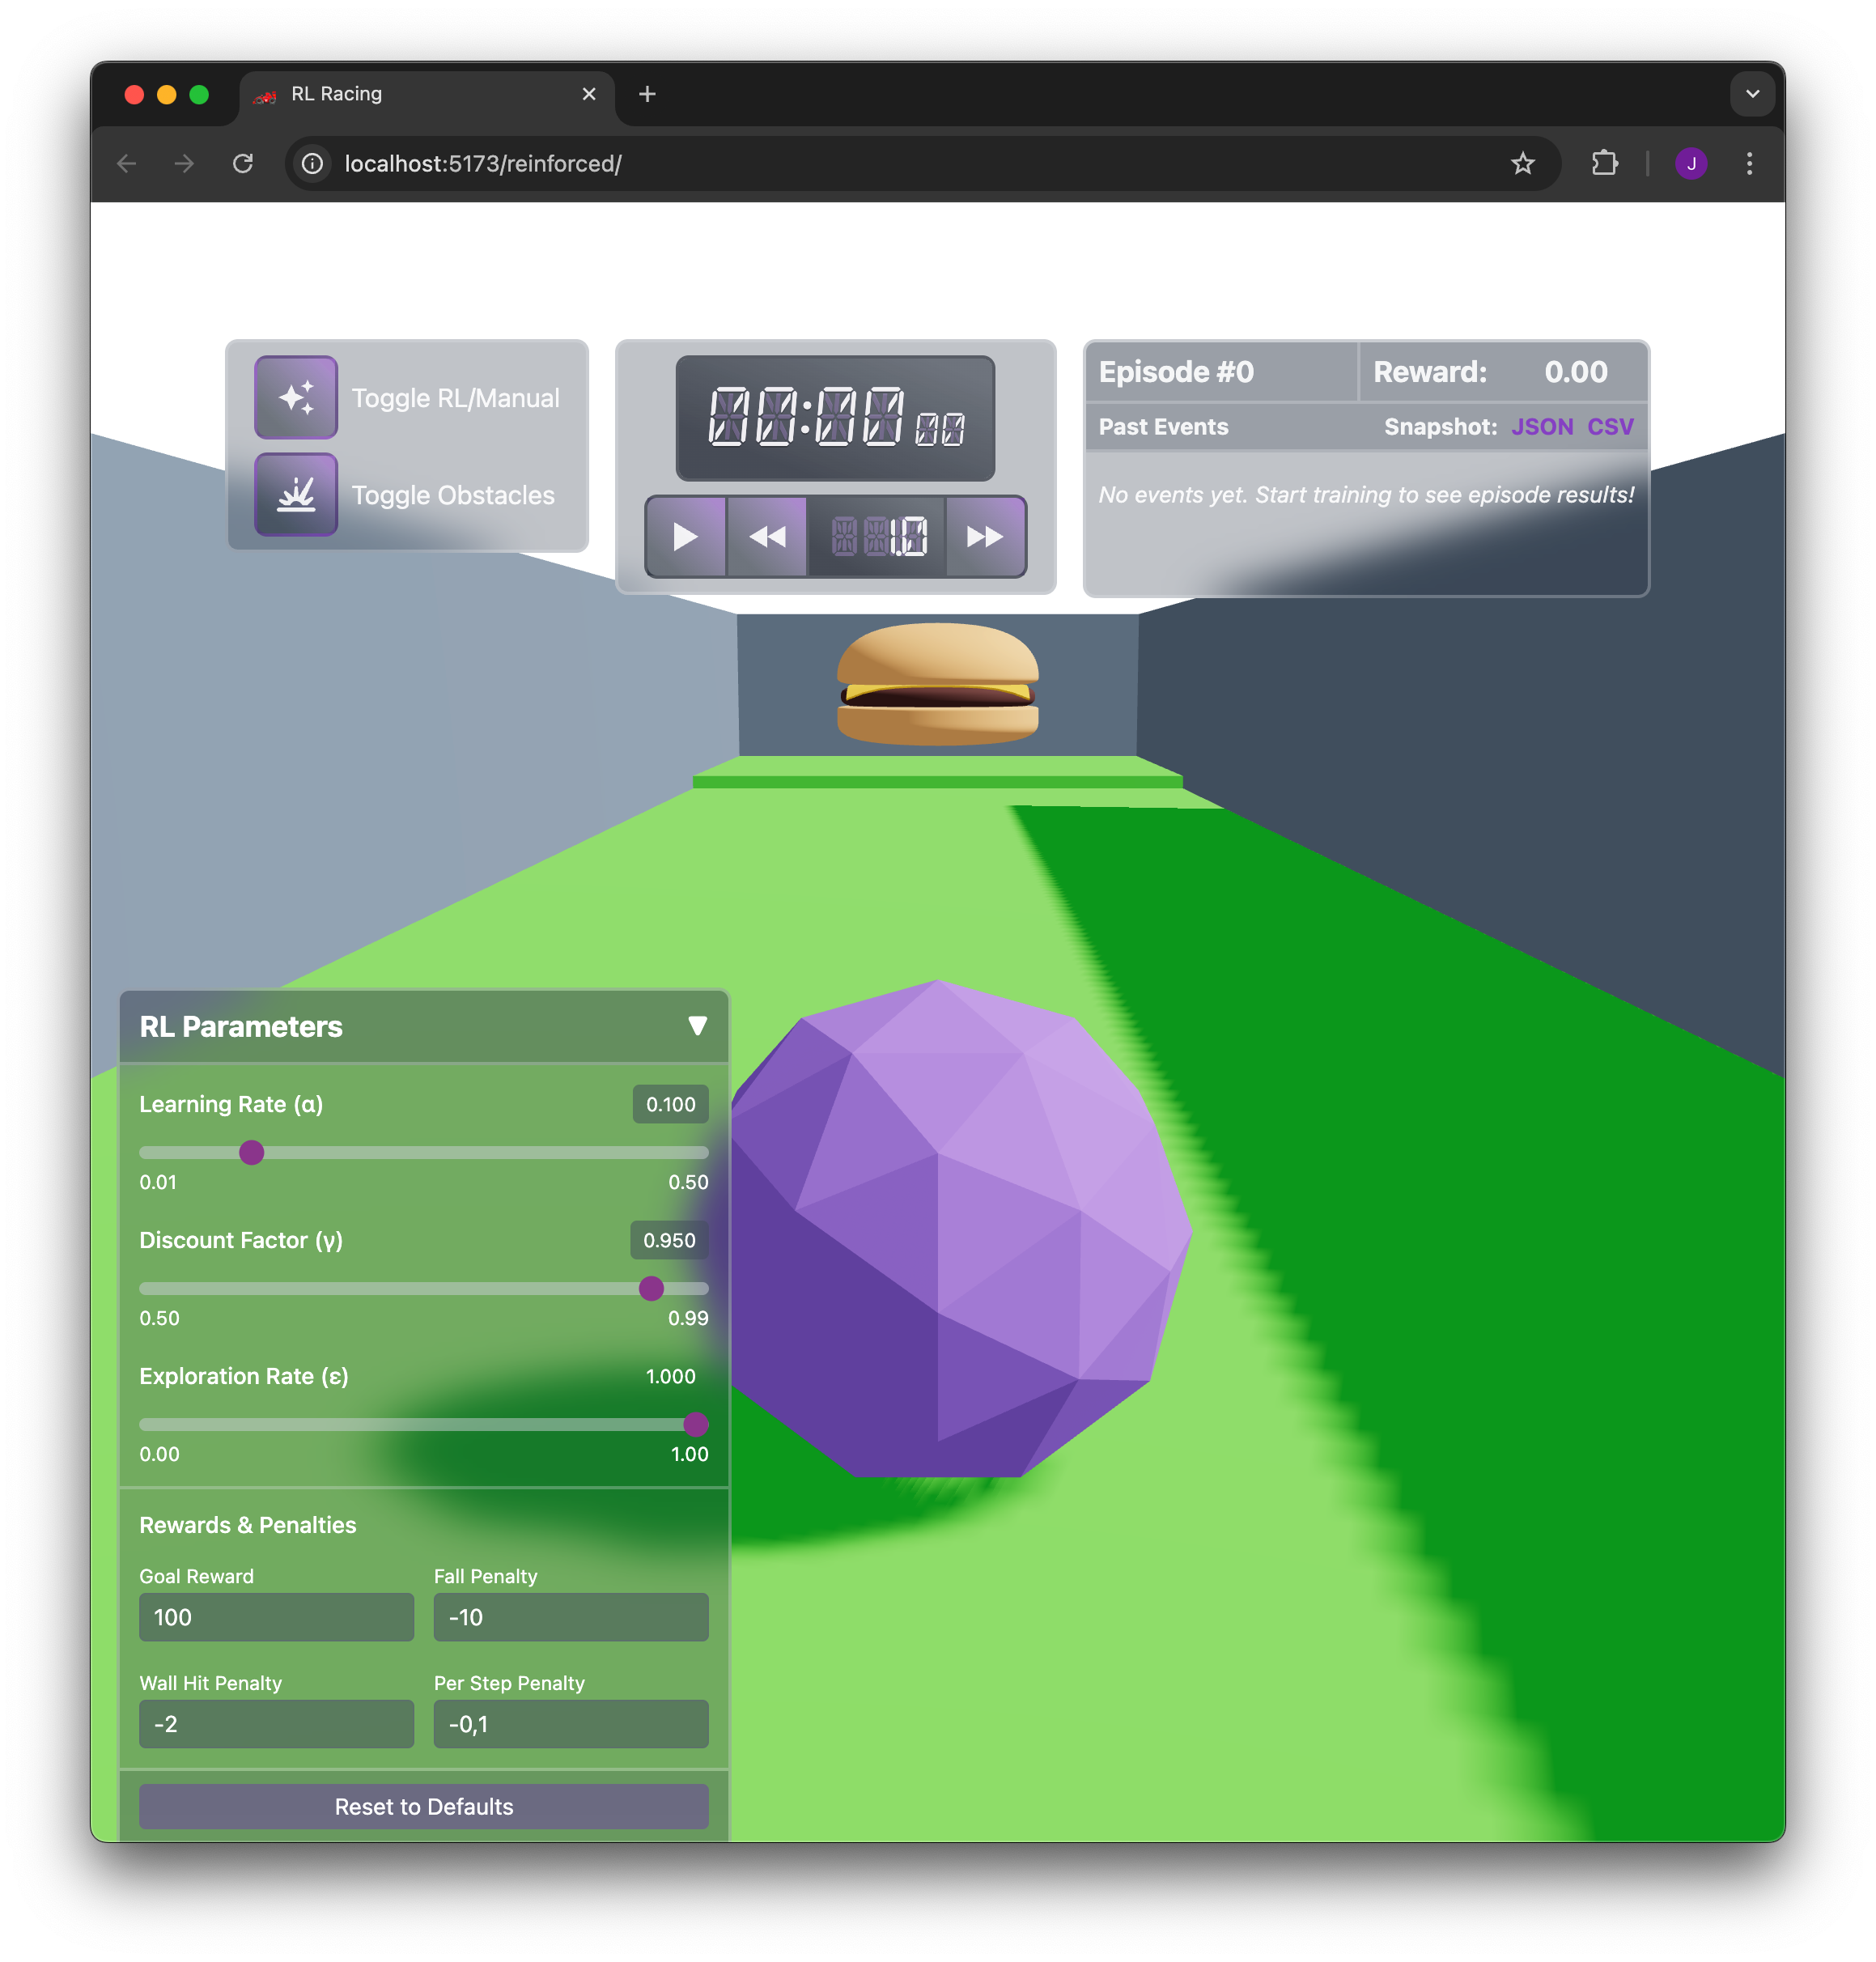
\includegraphics[width=0.45\textwidth]
    {figures/rl_racing_main.png}
    \caption{Final web application as seen on initial load.}
    \label{fig:rl_racing_main}
\end{figure}

The user interface was designed to provide intuitive control over fundamental reinforcement learning parameters and environmental conditions, enabling users to explore the impact of different configurations on agent behavior without requiring programming knowledge - Figure \ref{fig:rl_racing_main}.

\subsubsection{Real-time Monitoring Components}
A Timer component was implemented to display the duration of each episode in real-time. This component was initially designed as part of a broader simulation speed control system that would allow users to accelerate the learning process and observe long-term learning trends within compressed timeframes. However, due to technical complexity in synchronizing the physics simulation with variable time scales and project time constraints, the simulation speed control feature was not fully implemented in the final system.

The EventLogger component serves as a comprehensive monitoring system that displays real-time updates of total episode rewards alongside a chronological log of past episode outcomes. This component addresses the pedagogical need for immediate feedback by showing users the direct consequences of the agent's actions and parameter adjustments. The interface displays both the current episode's accumulated reward and a scrollable history of previous episodes, enabling users to identify learning trends and performance improvements over time.

\subsubsection{Dynamic Environment Control}
A critical educational feature of the interface is the obstacle toggle functionality, which allows users to enable or disable environmental obstacles at any point during the training process. This real-time environment modification capability demonstrates the impact of environmental complexity on learning performance, providing immediate visual evidence of how increased task difficulty affects agent behavior and learning progression.

\subsubsection{Data Export and Analysis Tools}
To facilitate deeper analysis of learning behavior, the system implements data export functionality that captures comprehensive training metrics in both JSON and CSV formats. The export system provides snapshot capabilities that allow users to download detailed learning data without interrupting the ongoing training process, preserving the real-time learning experience while enabling post-hoc analysis.
\section{Results}

The primary objective of this project was successfully achieved, demonstrating how fundamental reinforcement learning parameters and environmental conditions directly influence agent learning behavior. The developed browser-based environment effectively illustrates core RL concepts through real-time visualization and intuitive parameter control, enabling users to observe the exploration-exploitation trade-off without requiring programming expertise.

The experimental results clearly demonstrate the impact of environmental complexity on learning performance. Figure \ref{fig:performance_no_obstacles} shows optimal learning progression in a simplified environment, where the agent successfully transitions from exploration to exploitation, achieving consistent maximum rewards after approximately 100 episodes as epsilon decays appropriately.

\rlplot{data/rl_150_then_perfect.csv}{Learning progression without obstacles showing successful transition from exploration to exploitation}{fig:performance_no_obstacles}{-20}{105}

In contrast, Figure \ref{fig:performance_sudden_obstacles} illustrates the challenges of non-stationary environments when obstacles are introduced mid-training. The agent's performance degrades significantly after episode 100, yet the low epsilon value prevents renewed exploration, highlighting a fundamental limitation of fixed exploration strategies.

\rlplot{data/rl_100_clear_then_obstacles.csv}{Performance degradation when obstacles are introduced at episode 100, showing inadequate re-exploration}{fig:performance_sudden_obstacles}{-20}{105}

Figure \ref{fig:performance_all_obstacles} demonstrates the severe learning impairment when obstacles are present from initialization. Even after 500 episodes, the agent fails to achieve consistent success, with epsilon approaching zero despite poor performance.

\rlplot{data/rl_obsatcles_500.csv}{Learning failure with obstacles present from start, showing need for adaptive exploration}{fig:performance_all_obstacles}{-20}{105}
\section{Discussion}

These results underscore the need for adaptive exploration strategies in dynamic environments. Future work should implement adaptive epsilon functionality as a configurable option, allowing users to observe the benefits of exploration adjustment in response to environmental changes or performance degradation.

Additional enhancements could include more complex level designs featuring turns, branching paths, or multi-objective scenarios that would further emphasize the exploration-exploitation balance. Real-time plotting capabilities would also enhance the educational value by enabling direct comparison of different hyperparameter configurations during training, providing immediate visual feedback on parameter sensitivity and learning dynamics.

The system successfully bridges the gap between theoretical RL concepts and intuitive understanding through accessible visualization and parameter control, demonstrating the educational value of simplified, real-time learning environments.

\bibliographystyle{ieeetr}
\bibliography{biblio}

\end{document}
